% !Mode:: "TeX:UTF-8"
% +-----------------------------------------------------------------------------
% | File: pyneo4jet
% | Author: huxuan
% | E-mail: i(at)huxuan.org
% | Created: 2012-12-11
% | Last modified: 2012-12-11
% | Description:
% |     Report for pyneo4jet
% |
% | Copyrgiht (c) 2012 by huxuan. All rights reserved.
% | License GPLv3
% +-----------------------------------------------------------------------------

\documentclass{yaldc}

\title{Pyneo4jet 项目说明\\[2ex]\large基于Neo4j图形数据库的微博网站}
\author{
    \normalsize 扈\quad煊\qquad 1201214133 \\
    \normalsize 潘婉琼\qquad 1201214139 \\
    \normalsize 周\quad志\qquad 1201214118
}
\date{\today}

\begin{document}

\maketitle

\tableofcontents

\section{项目简介}

本项目是北京大学《海量图数据的管理与挖掘》的课程作业之一,主要是
利用开源的图数据库Neo4j来构建一个基本的社交网站。

\subsection{Neo4j}
Neo4j是一个用Java实现、完全兼容ACID的图形数据库。数据以一种针对图形网络进行
过优化的格式保存在磁盘上。Neo4j的内核是一种极快的图形引擎,具有数据库产品期
望的所有特性,如恢复、两阶段提交、符合XA等。

开发者可以通过Java-API直接与图形模型交互,这个API暴露了非常灵活的数据结构。
至于象JRuby/Ruby、Scala、Python、Clojure等其他语言,社区也贡献了优秀的绑定库。
本项目使用的是Neo4j基于Python的API。

Neo4j的典型数据特征:
\begin{itemize}
    \item 数据结构不是必须的,甚至可以完全没有,这可以简化模式变更和延迟数据
        迁移。
    \item 可以方便建模常见的复杂领域数据集,如CMS里的访问控制可被建模成细粒
        度的访问控制表,类对象数据库的用例、TripleStores以及其他例子。
    \item 典型使用的领域如语义网和RDF、LinkedData、GIS、基因分析、社交网络数
        据建模、深度推荐算法以及其他领域。
\end{itemize}

\subsection{Pyneo4jet}

\begin{description}
    \item[线上部署] \url{http://pyneo4jet.huxuan.org}
    \item[代码托管] \url{https://github.com/huxuan/pyneo4jet}
    \item[主要功能] ~
        \begin{itemize}
            \item 用户的注册、登录
            \item 用户资料/密码更新
            \item 好友的关注和取消关注
            \item 查看自己和好友的新鲜事
            \item 随便看看
        \end{itemize}
\end{description}

\section{项目分工}
本项目使用的是MVC(Model-View-Controller)模式,把软件系统分为三个基本
部分:模型(Model)、视图(View)和控制器(Controller)。

\subsection{模型层}

\begin{description}
    \item[负责人] 潘婉琼
    \item[编程语言] Python
    \item[代码文件] model.py
    \item[主要功能] 封装与Neo4j数据库的读写交互,实现主要设计的对象类及其方法
    \item[数据结构] User是用户类,提供用户与数据库的接口,
        包括用户的注册和登录验证、资料更新、关注和取消关注好友、
        得到自己的时间线、得到好友的新鲜事以及随便看看等;
        Tweet是消息类,提供消息与数据库的接口,包括新鲜事的新建和删除等。
\end{description}

\subsection{视图层}

\begin{description}
    \item[负责人] 周志
    \item[语言] Bottle 的模板语法(主要是HTML和Python的结合)
    \item[代码文件] views 目录下的所有文件,主要是tpl模板和css
    \item[主要功能] 对用户信息友好的展示,提供简洁方便的交互。
    \item[文件说明] Bottle是一种基于Python的快速、简单和轻量级的微web框架,
        通过对后缀为tpl的文件可实现模板的调用,通过route和控制回调实现对css
        文件的识别。其中base.tpl是基本模板,nav.tpl是导航栏模板,signin.tpl
        是登陆模板,signup.tpl是注册模板,tweet\_form.tpl是状态发布模板,
        profile.tpl是个人主页模板,password\_update.tpl是修改密码模板,
        profile\_update.tpl是更改个人信息模板,user.tpl是好友列表模板,
        style.css是网页的样式和布局。
\end{description}

\subsection{控制器层}

\begin{description}
    \item[负责人] 扈煊
    \item[编程语言] Python
    \item[代码文件] pyneo4jet.py
    \item[主要功能] 服务器端的指令处理以及和模型层、视图层的交互。
\end{description}

\subsection{数据解析脚本}

\begin{description}
    \item[负责人] 扈煊
    \item[编程语言] Python
    \item[代码文件] data/parser.py
    \item[主要功能] 解析原始数据,批量新建用户并利用用户信息模拟生成相应的消息。
\end{description}

\subsection{服务器相关}

\begin{description}
    \item[负责人] 扈煊
    \item[框架] Bottle \footnote{\url{http://bottlepy.org/}}
    \item[服务器] Gevent \footnote{\url{http://gevent.org/}}
    \item[反向代理] Nginx\footnote{\url{http://nginx.org/}}
    \item[说明] Bottle和Gevent都是基于Python并且非常轻量级,非常适合小项目使用,
        由于服务器上不止Pyneo4jet一个项目在运行,所以使用Nginx作为80端口的
        统一负载通过反向代理来实现Pyneo4jet的调用。
\end{description}

\subsection{工作量统计}

具体统计数据:\url{https://github.com/huxuan/pyneo4jet/graphs/contributors}

具体修改记录:\url{https://github.com/huxuan/pyneo4jet/commits/master}

\section{页面功能}

\subsection{/}

\begin{description}
    \item[网站首页] ~
    \item[功能说明] ~
        \begin{description}
            \item[GET] 默认跳转显示登录页面,如已登录则跳转到timeline,
                如果带有参数action=signup,则显示注册页面。
            \item[POST] 处理登录和注册请求,如出错则返回原页面并显示错误信息,
                否则跳转到timeline页面。
        \end{description}
\end{description}

\subsection{/<username>/}

\begin{description}
    \item[用户信息页面] ~
    \item[参数说明] ~
        \begin{description}
            \item[username] 当前浏览的用户名称
            \item[index] 消息列表开始编号
        \end{description}
    \item[功能说明] ~
        \begin{description}
            \item[GET] 默认显示用户信息页面,如果是当前登录用户则判断是否带有
                可能的action参数,如果参数action=profile\_update,
                则显示用户信息更新页面,如果参数action=password\_update,
                则显示用户密码更新页面。
            \item[POST] 如果是当前登录用户,则处理用户信息更新和密码更新的请求,
                根据action参数的不同进行不同的修改。如果不是当前用户,则处理关注
                和取消关注的请求,根据action参数等于follow还是unfollow
                进行用户之间关注关系的修改。
        \end{description}
\end{description}

\subsection{/<username>/timeline/<index:int>}

\begin{description}
    \item[用户新鲜事页面] ~
    \item[参数说明] ~
        \begin{description}
            \item[username] 当前浏览的用户名称
            \item[index] 消息列表开始编号
        \end{description}
    \item[功能说明] ~
        \begin{description}
            \item[GET] 获取当前浏览用户的信息列表,包括他和他好友最新的消息更新。
        \end{description}
\end{description}

\subsection{/<username>/tweets/<index:int>}

\begin{description}
    \item[用户消息页面] ~
    \item[参数说明] ~
        \begin{description}
            \item[username] 当前浏览的用户名称
            \item[index] 消息列表开始编号
        \end{description}
    \item[功能说明] ~
        \begin{description}
            \item[GET] 获取当前浏览用户发送的最新消息列表
        \end{description}
\end{description}

\subsection{/<username>/followers/<index:int>}

\begin{description}
    \item[关注用户者页面] ~
    \item[参数说明] ~
        \begin{description}
            \item[username] 当前浏览的用户名称
            \item[index] 用户列表开始编号
        \end{description}
    \item[功能说明] ~
        \begin{description}
            \item[GET] 显示关注当前浏览用户的用户列表
        \end{description}
\end{description}

\subsection{/<username>/following/<index:int>}

\begin{description}
    \item[用户关注者页面] ~
    \item[参数说明] ~
        \begin{description}
            \item[username] 当前浏览的用户名称
            \item[index] 用户列表开始编号
        \end{description}
    \item[] ~
        \begin{description}
            \item[GET] 显示当前浏览用户关注的用户列表
        \end{description}
\end{description}

\subsection{/<username>/random/}

\begin{description}
    \item[随便看看页面] ~
    \item[参数说明] ~
        \begin{description}
            \item[username] 当前浏览的用户名称
        \end{description}
    \item[] ~
        \begin{description}
            \item[GET] 获取非当前浏览用户所发的随机消息列表页面
        \end{description}
\end{description}

\section{Neo4j交互}

\begin{figure}[h!]
    \centering
    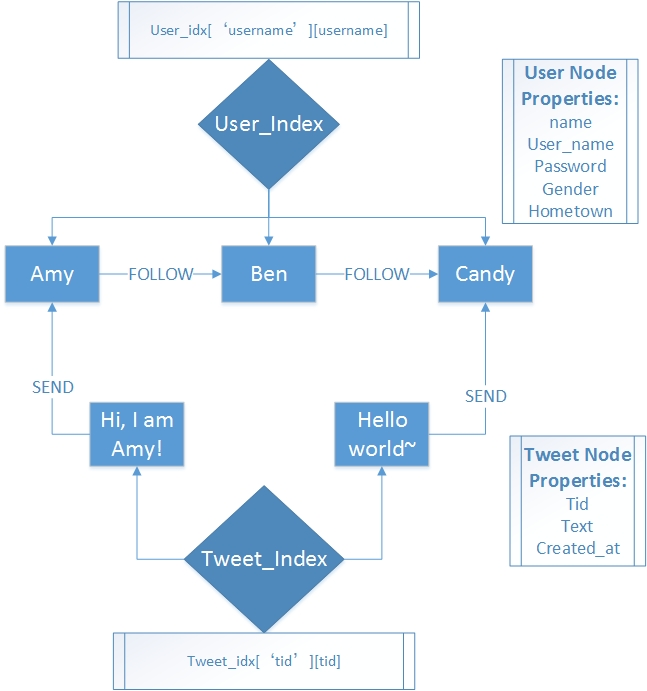
\includegraphics[width=.75\textwidth]{ds.jpg}
    \caption{数据结构}
    \label{fig-ds}
\end{figure}

\subsection{User}

\subsubsection{添加新用户到数据库}

\begin{description}
    \item[函数名] \verb|add(username, password, password_confirm, invitation)|
    \item[参数]
        \begin{description}
            \item[username] 用户名
            \item[password] 用户密码
            \item[password\_confirm] 用户密码确认
            \item[invitation] 邀请码
        \end{description}
    \item[步骤]
        \begin{enumerate}
            \item 判断该用户信息是否合法,如果不合法就返回False和错误信息。
            \item 新建一个user\_node,将参数中的的信息拷贝入user\_node中,
                并将该user\_node加入到用户索引user\_idx中。
            \item 创建成功,返回True。
        \end{enumerate}
    \item[代码] ~
        \begin{lstlisting}[language=Python]
if not username or not password or not password_confirm:
    return False, 'The username/password should not be empty!'
if password != password_confirm:
    return False, 'The password you input twice is not the same!'
if invitation != INVITATION_CODE:
    return False, 'The invitation code is invalid!'
user_node = user_idx['username'][username].single
if user_node:
    return False, 'The username %s has been used!' % username
with db.transaction:
    user_node = db.node()
    user_node['name'] = username
    user_node['username'] = username
    user_node['password'] = password
    user_idx['username'][username] = user_node
user = User.get(username)
return True, user
        \end{lstlisting}
\end{description}

\subsubsection{根据用户名找到对应的用户}

\begin{description}
    \item[函数名] \verb|get(username)|
    \item[参数]
        \begin{description}
            \item[username] 该用户的名称
        \end{description}
    \item[步骤]
        \begin{enumerate}
            \item 根据用户索引user\_idx找到所对应用户的user\_node。
            \item 新建一个User类,将user\_node的信息拷贝入user对象中。
            \item 返回User对象
        \end{enumerate}
    \item[代码] ~
        \begin{lstlisting}[language=Python]
user = None
user_node = user_idx['username'][username].single
if user_node:
    user = User(username, user_node['password'])
    user.name = user_node['name']
    user.gender = user_node['gender']
    user.hometown = user_node['hometown']
return user
        \end{lstlisting}
\end{description}

\subsubsection{关注好友}

\begin{description}
    \item[函数名] \verb|follow(self, username)|
    \item[参数]
        \begin{description}
            \item[username] 好友的用户名
        \end{description}
    \item[步骤]
        \begin{enumerate}
            \item 根据用户索引user\_idx找到self所对应用户的user\_node。
            \item 判断self用户是否已经follow了username用户,如果是的话,就返回False和错误信息。
            \item 根据用户索引user\_idx找到用户名为username所对应用户的follow\_user。
            \item 在user\_node和follow\_user之间建立FOLLOW关系,返回True。
        \end{enumerate}
    \item[代码] ~
        \begin{lstlisting}[language=Python]
user_node = user_idx['username'][self.username].single
for rel in user_node.FOLLOW.outgoing:
    f_node = rel.end
    if f_node['username'] == username:
        return False, 'You have followed %s !' % username
follow_user = user_idx['username'][username].single
with db.transaction:
    user_node.FOLLOW(follow_user)
return True, 'Follow user %s successfully!' % username
        \end{lstlisting}
\end{description}

\subsubsection{取消关注好友}

\begin{description}
    \item[函数名] \verb|unfollow(self, username)|
    \item[参数]
        \begin{description}
            \item[username] 好友的用户名
        \end{description}
    \item[步骤]
        \begin{enumerate}
            \item 根据用户索引user\_idx找到self所对应用户的user\_node。
            \item 判断self用户是否已经follow了username用户,如果是的话,
                就删除该关系,并返回True。
            \item 如果没有返回True的话,就在函数最后返回False。
        \end{enumerate}
    \item[代码] ~
        \begin{lstlisting}[language=Python]
user_node = user_idx['username'][self.username].single
with db.transaction:
    for rel in user_node.FOLLOW.outgoing:
        f_node = rel.end
        if f_node['username'] == username:
            rel.delete()
            return True, 'Unfollowed user %s!' % username
return False, 'You haven\'t follow %s yet !' % username
        \end{lstlisting}
\end{description}

\subsubsection{找到关注该用户的好友}

\begin{description}
    \item[函数名] \verb|get_followers(self, index=0, amount=10)|
    \item[参数]
        \begin{description}
            \item[index] 起始下标
            \item[amount] 需要返回的好友个数
        \end{description}
    \item[步骤]
        \begin{enumerate}
            \item 根据用户索引user\_idx找到self所对应的user\_from。
            \item 新建一个users\_list,将所有关注user\_from的好友加入该
                users\_list中。该步骤中主要用到了Neo4j中relationship的方向。
            \item 返回users\_list中满足下标条件的元素。
        \end{enumerate}
    \item[代码] ~
        \begin{lstlisting}[language=Python]
user_from = user_idx['username'][self.username].single
users_list = []
for relationship in user_from.FOLLOW.incoming:
    user_to = relationship.start
    user = User.get(user_to['username'])
    users_list.append(user)
return users_list[index : min(index+amount, len(users_list))]
        \end{lstlisting}
\end{description}

\subsubsection{找到该用户关注的好友}

\begin{description}
    \item[函数名] \verb|get_following(self, index=0, amount=10)|
    \item[参数]
        \begin{description}
            \item[index] 起始下标
            \item[amount] 需要返回的好友个数
        \end{description}
    \item[步骤]
        \begin{enumerate}
            \item 根据用户索引user\_idx找到self所对应的user\_from。
            \item 新建一个users\_list,将user\_from关注的所有好友加入该
                users\_list中。该步骤中主要用到了Neo4j中relationship的方向。
            \item 返回users\_list中满足下标条件的元素。
        \end{enumerate}
    \item[代码] ~
        \begin{lstlisting}[language=Python]
user_from = user_idx['username'][self.username].single
users_list = []
for relationship in user_from.FOLLOW.outgoing:
    user_to = relationship.end
    user = User.get(user_to['username'])
    users_list.append(user)
return users_list[index : min(index+amount, len(users_list))]
        \end{lstlisting}
\end{description}

\subsubsection{找到该用户发表的所有新鲜事}

\begin{description}
    \item[函数名] \verb|get_tweets(self, index=0, amount=10)|
    \item[参数]
        \begin{description}
            \item[index] 起始下标
            \item[amount] 需要返回的新鲜事个数
        \end{description}
    \item[步骤]
        \begin{enumerate}
            \item 根据用户索引user\_idx找到self所对应的user\_from。
            \item 新建一个tweets\_list,将user\_from发表的所有新鲜事都加入该
                tweets\_list中。该步骤中主要用到了Neo4j中relationship的方向。
            \item 返回tweets\_list中满足下标条件的元素。
        \end{enumerate}
    \item[代码] ~
        \begin{lstlisting}[language=Python]
user_from = user_idx['username'][self.username].single
tweets_list = []
for relationship in user_from.SEND.incoming:
    tweet_node = relationship.start
    tweet = Tweet()
    tweet.text = tweet_node['text']
    tweet.username= tweet_node.SEND.outgoing.single.end['username']
    tweet.created_at = tweet_node['created_at']
    tweet.tid = tweet_node['tid']
    tweets_list.append(tweet)
tweets_list.sort(key=lambda tweet: tweet.created_at, reverse=True)
return tweets_list[index : min(index + amount, len(tweets_list))]
        \end{lstlisting}
\end{description}

\subsubsection{返回该用户及其好友的新鲜事列表}

\begin{description}
    \item[函数名] \verb|get_timeline(self, index=0, amount=10)|
    \item[参数]
        \begin{description}
            \item[index] 起始下标
            \item[amount] 需要返回的新鲜事个数
        \end{description}
    \item[步骤]
        \begin{enumerate}
            \item 根据用户索引user\_idx找到self所对应的user\_node。
            \item 新建一个tweets\_list,将user\_node及其好友发表的所有新鲜事都加
                入该tweets\_list中。该步骤中主要用到了Neo4j中relationship的方向。
            \item 对tweets\_list按创建时间进行排序
            \item 返回tweets\_list中满足下标条件的元素。
        \end{enumerate}
    \item[代码] ~
        \begin{lstlisting}[language=Python]
tweets_list = []
user_node = user_idx['username'][self.username].single
for follow_rel in user_node.FOLLOW.outgoing:
    follow_node = follow_rel.end
    for send_rel in follow_node.SEND.incoming:
        tweet_node = send_rel.start
        tweet = Tweet.get(tweet_node['tid'])
        tweets_list.append(tweet)
for rel in user_node.SEND.incoming:
    tweet_node = rel.start
    tweet = Tweet.get(tweet_node['tid'])
    tweets_list.append(tweet)
tweets_list.sort(key=lambda tweet: tweet.created_at, reverse=True)
return tweets_list[index : min(index + amount, len(tweets_list))]
        \end{lstlisting}
\end{description}

\subsubsection{随便看看,返回非该用户的随机新鲜事}

\begin{description}
    \item[函数名] \verb|get_random_tweets(self, index=0, amount=10)|
    \item[参数]
        \begin{description}
            \item[index] 起始下标
            \item[amount] 需要返回的新鲜事个数
        \end{description}
    \item[步骤]
        \begin{enumerate}
            \item 从tweet\_ref处获得当前的tweet总个数tot。
            \item 新建一个random\_list,和变量count初始化为0。
            \item 在(0,tot)中随机生成一个tid,判断该tid对应的tweet的用户是否
                为self,如果不是的话,就判断rancom\_list中是否已经加入该tweet,
                如果没有加入过的话,就把该tweet加入random\_list中。
                Count记录的是循环的次数。
            \item 重复上一步,直到random\_list中的元素大于等于amount
                或者count大于10倍的amount。
            \item 返回random\_list。
        \end{enumerate}
    \item[代码] ~
        \begin{lstlisting}[language=Python]
tot = tweet_ref['tot_tweet']
random_list = []
tids = set([])
count = 0
while(len(random_list) < amount):
    count += 1
    tid = random.randrange(0, tot)
    tweet = Tweet.get(tid)
    if tweet.username != self.username and tid not in tids:
         random_list.append(tweet)
         tids.add(tid)
    if count > 10 * amount:
         break
random_list.sort(key=lambda tweet: tweet.created_at, reverse=True)
return random_list
        \end{lstlisting}
\end{description}

\subsection{Tweet}

\subsubsection{添加新鲜事到数据库}

\begin{description}
    \item[函数名] \verb|add(username, text, created_at)|
    \item[参数]
        \begin{description}
            \item[username] 发表该tweet的用户
            \item[text] tweet内容
            \item[created\_at] tweet创建时间
        \end{description}
    \item[步骤]
        \begin{enumerate}
            \item 根据用户索引user\_idx找到username所对应的用户的user\_node,
                新建一个tweet\_node,将该tweet\_node与user\_node之间建立一个
                SEND关系。
            \item 根据数据库中的tweet\_ref点得到目前tweet的总个数N,然后给该
                tweet分配一个新的tid(N+1)。
            \item 将tweet\_node加入到tweet索引tweet\_idx中。
        \end{enumerate}
    \item[代码] ~
        \begin{lstlisting}[language=Python]
user_node = user_idx['username'][username].single
if not user_node:
    return False, 'User not found!'
if text:
    with db.transaction:
        tweet_node = db.node()
        tweet_node['text'] = text
        tweet_node['created_at'] = created_at
        tweet_node.SEND(user_node)
        tid = tweet_ref['tot_tweet']
        tweet_node['tid'] = tid
        tweet_ref['tot_tweet'] = tweet_ref['tot_tweet'] + 1
        tweet_idx['tid'][tid] = tweet_node
        return True, ''
else:
return False, 'Tweet should not be empty!'
        \end{lstlisting}
\end{description}

\subsubsection{根据tid找到对应的tweet}

\begin{description}
    \item[函数名] \verb|get(tid)|
    \item[参数]
        \begin{description}
            \item[tid] 该tweet的编号
        \end{description}
    \item[步骤]
        \begin{enumerate}
            \item 根据tweet索引tweet\_idx找到tid所对应的tweet的tweet\_node。
            \item 新建一个Tweet() tweet,将tweet\_node的信息拷贝入tweet对象中。
            \item 返回tweet
        \end{enumerate}
    \item[代码] ~
        \begin{lstlisting}[language=Python]
tweet = Tweet()
tweet_node = tweet_idx['tid'][tid].single
if tweet_node:
    tweet.username = tweet_node.SEND.outgoing.single.end['username']
    tweet.text = tweet_node['text']
    tweet.created_at = tweet_node['created_at']
    tweet.tid = tweet_node['tid']
    return tweet
        \end{lstlisting}
\end{description}

\section{心得体会}

\subsection{周志}

通过本次实验,我学习了python的有关知识,尤其是基于python的web框架bottle,
对git,github版本管理有了简单的认识,进一步学习了html和css的相关知识,
对网页布局和美化有了更深的了解。

在本次实验中,我对团队协调的有了更深的认识,刚开始考虑事情不够周全,
在项目规范和开发工具使用上犯了一些错误,经过和组员交流我意识到了问题的严重性
,对此在以后的项目开发上这个问题值得重视。

在本次实验中我要感谢两位组员在我遇到困难时给予的帮助和支持以及
在我给项目增添麻烦时给予的理解和包涵。

\subsection{潘婉琼}

经过本次实验,我对图数据库有了更深入的理解,
发现了图数据库与关系数据库的根本性不同,图数据库比关系数据库要灵活很多。

在编程的过程中,我学习了在Linux环境下使用python脚本语言进行编程和调试,
并学会了GIT版本控制软件的简单使用方法。

在此要特别感谢扈煊同学对我耐心的帮助和指导,从他身上,
我学到了很多程序员应该具备的专业素质。

\subsection{扈煊}

Pyneo4jet实现了一个简单的微博网站所必须的基本功能,主要特色是用Neo4j图数据库
代替了常规的关系型数据库如MySQL用于数据的存取,整个网站的控制层和视图层几乎
没有涉及Neo4j的交互,所有与Neo4j的交互都由模型层封装成了相应的类和方法,这也
是为什么本项目使用MVC三层架构模式的主要原因。

在使用图数据库的过程中,比较重要的一点是抛弃已经熟悉的关系型数据库的思维,尽
可能的理解不同的NoSQL系统特有的特点和优势,例如Neo4j的索引和id概念,neo4j的
索引本质上就是一个key-value的hash,id在neo4j中也不是必要的元素,在Pyneo4jet
中User的存取就直接将username作为key而且没有存储任何额外的类似于id的元素。此
外在保存user及其所发的tweet以及user之间的follow关系时,使用的是Neo4j的relati
onship而不必再使用额外的表来记录这些关系,这不仅简化了数据之间的逻辑,而且让
代码也更加具有易读性,应该说正是Neo4j的精华所在。

与此同时,Neo4j也有很多可以改进的地方,比如需要额外人工维护的索引是一个非常大的硬伤,
应该至少支持某种规则的索引,这个规则可以是特定type的relationship,例如friends
关系,也可以是特定type的node的properties的key,例如user的username,然后将这
一类规则的索引由系统自身维护,从而进一步增加Neo4j的集成度并减少Neo4j的使用者
也就是开发者的工作。

在团队交流中,主要由于我的个人习惯,让另外两位队友都使用了git/github版本管理、
python语言以及bottle模块,可能是由于对这些工具接触不久,所以不少时间都用在了
项目本身以外问题的沟通上,我切实感受到了两位队友短时间内在这些方面都有了很大
的提升,在此也为在交流过程中由于自身性格原因有时过于生硬的言辞表示歉意,
很高兴与你们一起顺利完成本次大作业。

当然,Pyneo4jet作为本次课程的大作业,离真正的实用还有很大的差距,由于事先未能
进行足够完备的设计,项目实现过程也过于仓促,尤其是控制器部分的内容,基本没有
Code Review,差不多都是以可以运行作为标准,难免很多缺漏的地方,甚至可能有跨站攻击
的潜在危险,我们尽可能的将代码尤其是安全性方面进行了完善,并且部署在线上
供老师、助教和其他同学亲身体验,如发现任何bug或者是任何建议,还望不吝指出。

\begin{thebibliography}{9}
    \bibitem[1]{neo4j} Neo4j 说明文档,
        \url{http://docs.neo4j.org/chunked/stable/index.html}
    \bibitem[2]{neo4jpytut} Neo4j python wrapper 简明文档,
        \url{http://docs.neo4j.org/chunked/stable/tutorials-python-embedded.html}
    \bibitem[3]{neo4jpy} Neo4j python wrapper 文档,
        \url{http://docs.neo4j.org/chunked/stable/python-embedded.html}
    \bibitem[4]{abop} Swaroop, C. H. "A Byte of Python.", 2003.
    \bibitem[5]{python} Python 官方文档 (Python 2.7),
        \url{http://docs.python.org/2.7/}
    \bibitem[6]{bottle} Bottle简明文档,
        \url{http://bottlepy.org/docs/stable/tutorial.html}
    \bibitem[7]{bottlestpl} Bottle 模板语法说明文档,
        \url{http://bottlepy.org/docs/stable/stpl.html}
    \bibitem[8]{html} W3School HTML 教程,
        \url{http://www.w3school.com.cn/html/}
    \bibitem[9]{css} W3School CSS 教程,
        \url{http://www.w3school.com.cn/css/}
\end{thebibliography}

\end{document}
